\documentclass[12pt]{article}

\usepackage[margin=0.8 in]{geometry}
\usepackage{amsmath}
\usepackage{amssymb}
\usepackage{macros}
\usepackage{mathtools}
\usepackage{enumerate}
\usepackage{verbatim}
\usepackage{amsthm}

\title{}
%\content{}



\let \proj \undefined
\renewcommand{\tr}{ \mathrm{tr}}
\DeclareMathOperator{\SU}{SU}
\DeclareMathOperator{\proj}{proj}
\newcommand{\sS}{\mathscr{S}}
\DeclareMathOperator{\comp}{comp}
\newcommand{\A}{\mathcal{A}}
\renewcommand{\D}{\mathcal{D}}
\renewcommand{\e}{\epsilon}
\newcommand{\Are}{\A_{r,\e}}
\newcommand{\Kre}{K_{r,\e}}
\newcommand{\Dre}{\D_{r,\e}}
\newcommand{\rt}{\tilde{r}}
\newcommand{\et}{\tilde{\e}}
\newtheorem{definition}{Definition}
\newenvironment{solution}
  {\begin{proof}[Solution]}
  {\end{proof}}
\newtheorem{example}{Example}
\newtheorem{exercise}{Exercise}
\newtheorem{theorem}{Theorem}


\newcommand{\vr}{\mathbf{r}}
\newcommand{\vF}{\mathbf{F}}



\begin{document}
\section*{15.3. Double Integrals over general regions and Properties}
Goals from this section:
\begin{enumerate}
\item Be able to compute double integrals over general regions by switching the order of integration if necessary (see Remark (2) on p.3).
\item Be comfortable using the properties of double integrals.
\item Know the definition of the average value of a function of two variables.
\end{enumerate}
In the previous section we saw how to integrate over rectangles using Fubini's theorem. Now we'll see how to integrate over more general regions and we'll see two such types of regions. In practice, a given region may not fall under any of those categories, but splitting it into smaller subregions will allow us to perform the integration.

\vspace{.1 in}

**The following discussion gives the definition of the integral over a general bounded region, and is a bit technical. If you find it too confusing you may ignore it and proceed to the theorems.

\textbf{Question:} What is the integral over a more general bounded region $D$? Do we need to go through Riemann sums again to make sense of it?

\textbf{Answer:} No! We can use our already existing definition, and a tool called a characteristic function. If $D$ is a region on the $xy$-plane, the characteristic function $\chi_D$ of $D$ is given by $$\chi_D(x,y)=\begin{cases}
1, & \text{ if }(x,y)\in D \\
0, &\text{ if }(x,y)\notin D
\end{cases}.$$
Then, if $R$ is a rectangle such that $D\subset R$, we define $$\iint_D f(x,y)dA:= \iint_R \chi_D(x,y) f(x,y)dA.$$ Note that the function $\chi_D(x,y) f(x,y)$ is not necessarily continuous! However, for a reasonable (not pathological) domain $R$ this is not a problem. For this class, pretty much everything we'll have to deal with is not going to be pathological and we won't have to worry too much about it. 

Even though this is how we define the integral over $D$, it's not how we do calculations in practice.

\subsection*{1st case}
\begin{theorem} Suppose we have a region that can be described as $$D=\{ (x,y):a\leq x \leq b, g_1(x)\leq y\leq g_2(x)\},$$ where $g_1$ and $g_2$ are continuous functions, and a continuous function $f(x,y)$ defined on $D$. Then we have: $$\iint_D f(x,y) dA =\int_a^b \int_{g_1(x)}^{g_2(x)} f(x,y)dy dx.$$
\end{theorem}
An example of such a region:

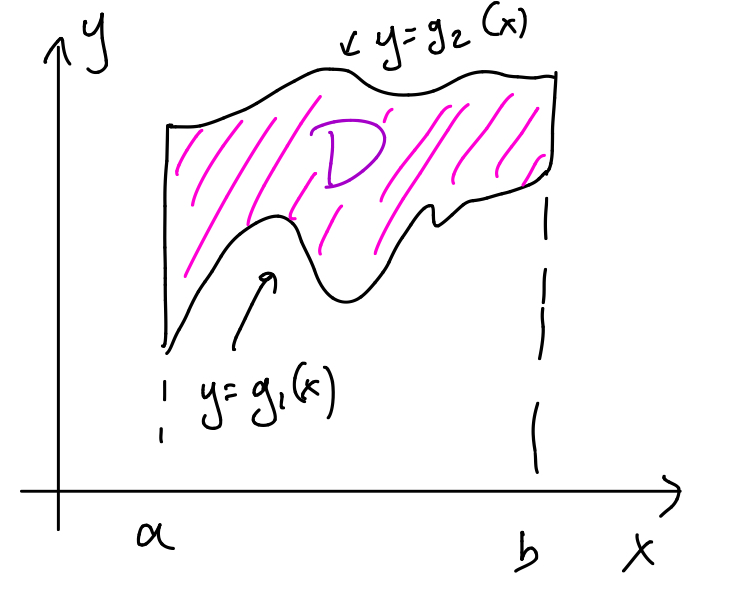
\includegraphics[scale=.2]{type_1.jpeg}
\begin{example}
Let $D$ be the domain bounded by $y=0$, $y=x^2$ and $x=1$. Find $\iint_D x\cos(y) dA$. 
\end{example}
\begin{solution}
Let's draw a picture: 

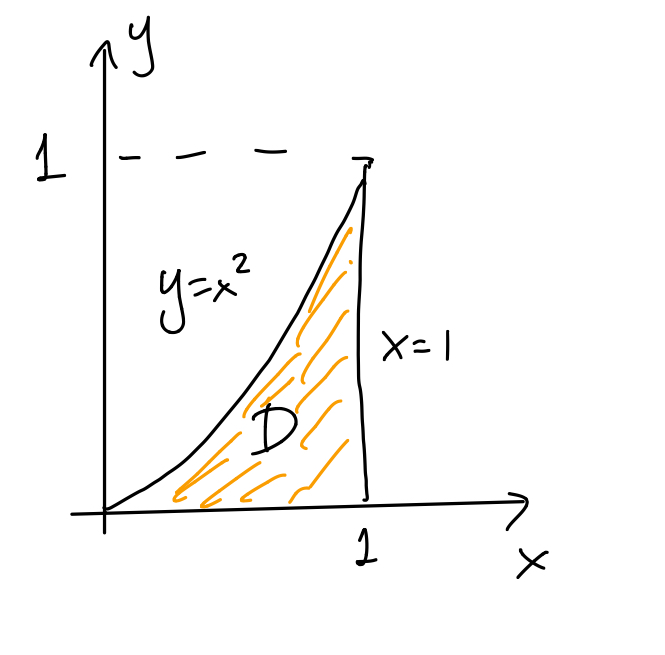
\includegraphics[scale=.2]{example.jpeg}
Note that $$D=\{ (x,y):0\leq x \leq 1, 0\leq y\leq x^2\},$$ so by our theorem$$\iint_D x\cos(y) dA=\int_0^1\int_0^{x^2} x\cos(y)dy dx=\dots=\frac{1}{2}(1-\cos(1)).$$

\end{solution}


\subsection*{2nd case}
\begin{theorem} Suppose we have a region that can be described as $$D=\{ (x,y): h_1(y)\leq x\leq h_2(y), c\leq y\leq d \},$$ where $h_1$ and $h_2$ are continuous functions, and a continuous function $f(x,y)$ defined on $D$. Then we have: $$\iint_D f(x,y) dA =\int_c^d \int_{h_1(x)}^{h_2(x)} f(x,y)dx dy.$$
\end{theorem}
An example of such a region:

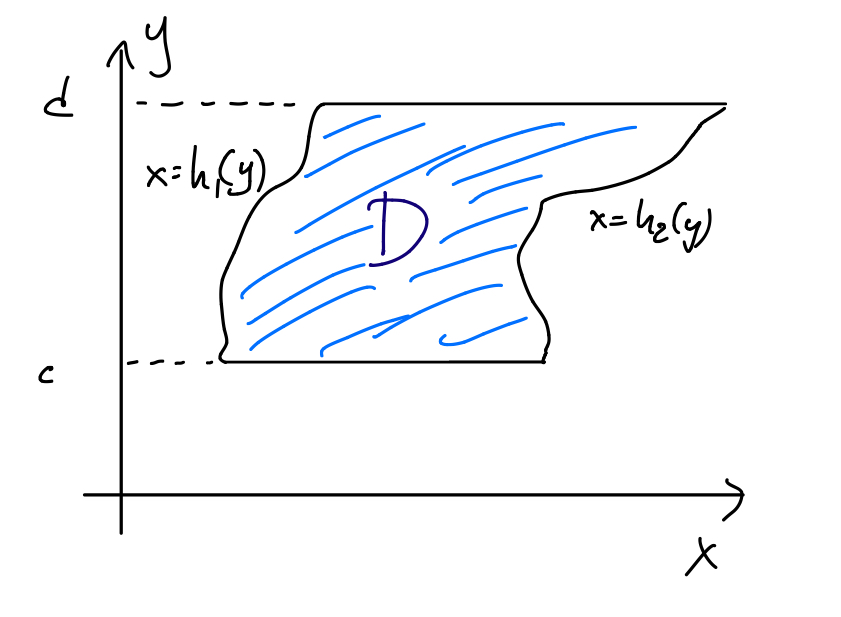
\includegraphics[scale=.2]{type_2.jpeg}

\textbf{Remark: }Note that the order of $dx$ and $dy$ is reversed compared to Theorem 1!

\begin{example} Same question as in Example 1.  
\end{example}
\begin{solution} Note that we may describe $D$ as $$D=\{ (x,y): \sqrt{y}\leq x\leq 1, 0\leq y\leq 1 \}$$ and therefore $$\int_D x\cos(y) dA =\int_0^1\int_{\sqrt{y}}^1 x\cos(y) dx dy=\dots=\frac{1}{2}(1-\cos(1)).$$

\end{solution}






\textbf{Remarks:} \begin{enumerate}
\item If a domain can be written in both ways, the result has to be the same regardless of whether we use theorem 1 or 2 for the computation. You can often use this idea to check your answer.
\item In Real Life\footnote{Real Life in this context means homework and exams}, if an integral can be written both ways, one of them is very hard or impossible to calculate, so you need to change the order of integration and the bounds.
\item As we're expecting to find a number as an answer, the bounds on the outer integral have to be constant regardless of the order of integration.

\end{enumerate}

\subsection*{Properties of double integrals}
Here $f$, $g$ are continuous functions and $D$ is a bounded region. You might find those properties obvious, but it's good to be mentioned.
\begin{enumerate} 
\item If $D=D_1 \cup D_2$ and $D_1,D_2$ don't overlap except maybe at their boundaries, then $$\iint_D f(x,y) dA=\iint_{D_1}f(x,y)dA + \iint_{D_2}f(x,y) dA.$$
\item $$\iint_Df(x,y)+g(x,y)dA=\iint_D f(x,y)dA +\iint_D g(x,y)dA.$$
\item If $c$ is \textbf{constant}, $$\iint_D cf(x,y) dA=c\iint_D f(x,y) dA$$
\item If $f(x,y)\leq g(x,y)$ for all $(x,y)\in D$ then $$\iint_D f(x,y)dA\leq \iint_D g(x,y) dA.$$
\item If $A(D)$ denotes the area of $D$, $$\iint_D1dA=A(D).$$ 
\end{enumerate}


\textbf{Remarks:}
\begin{enumerate}
\item Property (1) is important because it allows us to calculate integrals over regions that can't be written in either of the two ways described in Theorems 1 and 2. Here's a picture of such a region:

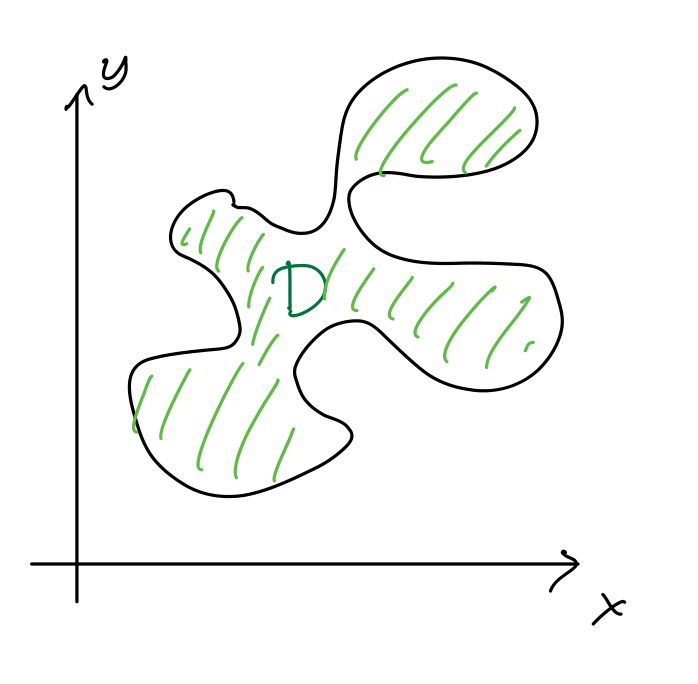
\includegraphics[scale=.2]{bad.jpeg}

Here's another occasion where this property is important: Let $D$ be the region described as $$D=\{(x,y):0\leq x\leq 1, x^2\leq y\leq 2\}.$$ If Real Life asked you to set up an integral on $D$ in the order $dxdy$ how would you do it?

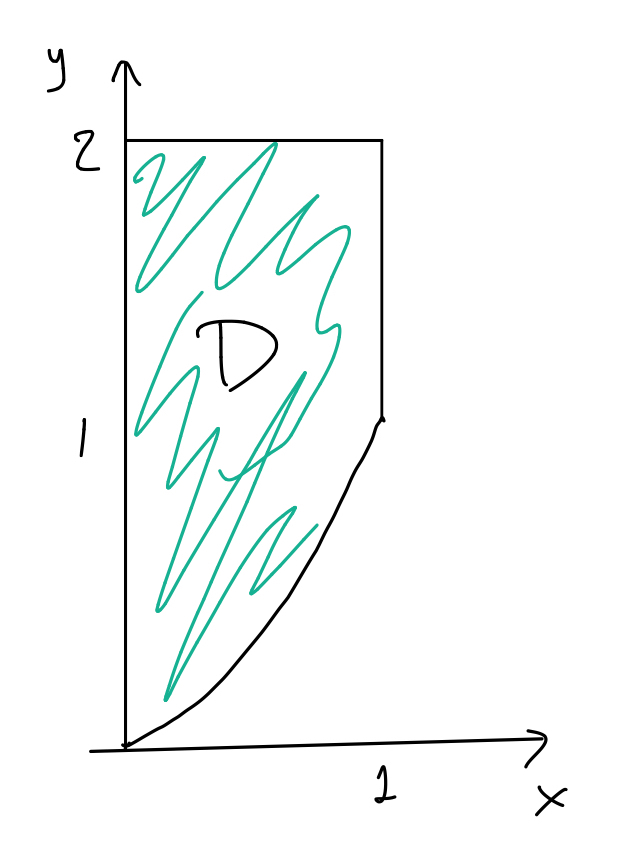
\includegraphics[scale=.2]{change.jpeg}

\item Property (4) is one of the most fundamental and most frequently used in Mathematical Analysis. Very often we don't care or can't compute the exact value of an integral of a function $f$ over a domain $D$, but we can find a function $g$ that can be easily integrated and has the property that $f\leq g$ on $D$ or $g\leq f$ on $D$ and this allows us to find an estimate on $\iint_D f(x,y)dA$.

\begin{exercise} Show that if $m\leq f(x,y)\leq M$ on $D$, with $m, M$ constants, then $$mA(D)\leq \iint_D f(x,y)dA\leq MA(D).$$
\end{exercise}

\begin{exercise} Show that if $D_1\subset D_2$ and $f\geq 0$ on $D_2$ then $$\iint_{D_1}f(x,y)dA\leq \iint_{D_2}f(x,y)dA.$$ 
\end{exercise}
\begin{exercise} Show that $$|\int_D f(x,y)dA|\leq \int_D |f|(x,y)dA,$$ where $|a| $ denotes the absolute value of $a$.\end{exercise}
(you may apply the properties without worrying about continuity issues)

\end{enumerate}

\subsection*{The average value}
One of the most important objects defined using integrals is the average value.
\begin{definition} If a continuous function $f(x,y)$ is defined on a region $D$ with area $A(D)$, the \textbf{average value} of $f$ is $$f_{ave}:= \frac{1}{A(D)}  \iint_D f(x,y) dA.$$
\end{definition}
Often in mathematics, we might not have know exactly the value of a function at every point, but we might have information about the average value of $f$, and this allows us to extract information about $f$.

\begin{exercise}
If $f_{ave}< M$ for a continuous function $f$ on a domain $D$, show that there exists at least a point $(x,y)\in D$ such that $f(x,y)<M$.
\end{exercise}


\end{document}
